\documentclass{article}

% ── arXiv preprint ──
\usepackage[preprint]{neurips_2026}

\usepackage[utf8]{inputenc}
\usepackage[T1]{fontenc}
\usepackage{hyperref}
\usepackage{url}
\usepackage{booktabs}
\usepackage{amsmath}
\usepackage{amssymb}
\usepackage{graphicx}
\usepackage{enumitem}
\usepackage{natbib}
\usepackage{xcolor}

\title{Do LLMs Know What They Know? \\Measuring Metacognitive Efficiency with Signal Detection Theory}

\author{%
  Jon-Paul Cacioli \\
  Independent Researcher \\
  Melbourne, Australia \\
  \texttt{synthium@hotmail.com} \\
  ORCID: 0009-0000-7054-2014
}

\begin{document}

\maketitle

\begin{abstract}
Standard evaluation of LLM confidence relies on calibration metrics (ECE, Brier score) that conflate two distinct capacities: how much a model knows (Type-1 accuracy) and how well its confidence signal tracks that knowledge (Type-2 metacognitive sensitivity). We apply Signal Detection Theory (SDT) to decompose these capacities in large language models, treating token-level normalised log-probability as a graded confidence variable and answer correctness as the state to be discriminated. We characterise the Type-2 ROC of this signal, including its unequal-variance structure via z-ROC analysis, and---because the meta-$d'$ efficiency ratio is not well defined for open-ended QA, which lacks a two-alternative Type-1 decision---quantify metacognitive efficiency with a model-free information measure, normalised metacognitive information (meta-$I_{2r}$). Applied to four LLMs (Llama-3-8B-Instruct, Mistral-7B-Instruct-v0.3, Llama-3-8B-Base, Gemma-2-9B-Instruct) across 224{,}000 factual QA trials, we find: (1)~metacognitive information varies more than two-fold across models and is decoupled from accuracy---Mistral achieves the lowest accuracy yet the highest metacognitive information, while Gemma-2, the most accurate, has the lowest; this ordering replicates on Natural Questions; (2)~the confidence signal has model-specific unequal-variance structure (z-ROC slopes from 0.81 to 1.18) that is invisible to calibration metrics; (3)~metacognitive information is domain-specific, strongest in Arts \& Literature for every model; (4)~temperature dissociates Type-1 accuracy from metacognitive information, which stays stable while accuracy shifts. All estimates carry permutation nulls and bootstrap confidence intervals. Pre-registered analysis; code and data publicly available.
\end{abstract}

\footnotetext[1]{\textbf{Version note (v2).} An earlier version of this paper estimated metacognitive efficiency using meta-$d'$/$M$-ratio. That estimator requires a two-alternative Type-1 detection decision, which open-ended factual QA does not provide; forcing the mapping makes $d'$ and meta-$d'$ functions of the same correctness-by-confidence table, so $M$-ratio is pinned near 1 by construction and reported cross-model $M$-ratio differences reflect departures from the equal-variance assumption rather than metacognitive efficiency. This version replaces $M$-ratio throughout with a model-free measure (meta-$I_{2r}$) and reports the Type-2 SDT structure (AUROC$_2$, z-ROC slope, $d_a$) directly. All analyses were re-run on the same 224{,}000-trial dataset. The domain-specificity and temperature-dissociation findings are unchanged; the direction of the cross-model efficiency finding reverses under the corrected measure.}

% ════════════════════════════════════════════════════════════════
\section{Introduction}

When a large language model (LLM) answers a factual question, two capacities determine the reliability of its output: its ability to discriminate correct from incorrect responses, and its ability to \emph{monitor} that discrimination through its confidence signal. These are fundamentally different problems requiring different interventions. A model that cannot discriminate needs better training data or architectural improvements. A model that discriminates well but monitors poorly needs recalibration, not retraining. Current evaluation practice does not make this distinction.

Consider two hypothetical models evaluated on the same factual QA benchmark. Model~A reports 90\% confidence on every trial and achieves 90\% accuracy; its Expected Calibration Error (ECE) is near zero. Model~B reports 95\% confidence when correct and 60\% when incorrect, but its average confidence overshoots its 80\% accuracy; its ECE is worse than Model~A's. Yet Model~B's confidence is \emph{far more useful}: it tells you which specific answers to trust. Model~A's confidence, despite perfect calibration, carries no information about correctness. The standard ECE metric rewards the wrong model.

This example illustrates a well-known limitation of ECE~\citep{guo2017calibration}: it measures the average alignment between confidence and accuracy, conflating the \emph{resolution} of the confidence signal (how well it separates correct from incorrect) with its \emph{bias} (the overall level of confidence). The Brier score decomposes into reliability, resolution, and uncertainty, but not into the model's discriminative capacity and its metacognitive sensitivity controlling for that capacity. The Area Under the Type-2 ROC (AUROC$_2$) of the confidence--accuracy curve~\citep{steyvers2025metacognition} improves on ECE by measuring ranking quality, but does not normalise for the base rate of correct responses, so it is not directly comparable across models of different accuracy.

Signal Detection Theory (SDT; \citealt{green1966signal}; \citealt{macmillan2005detection}) provides the natural framework for this decomposition. Developed over seven decades of psychophysical research, SDT separates performance into \emph{sensitivity} (how well an observer discriminates two states) and \emph{criterion} (the observer's threshold for responding). \citet{cacioli2026llms} demonstrated that the parametric SDT framework---ROC analysis, unequal-variance model fitting, criterion estimation---reveals structure in LLM confidence invisible to calibration metrics alone.

The present work applies SDT at the \emph{Type-2} level: how well does a model's confidence signal discriminate its own correct from incorrect answers? We treat token-level normalised log-probability (NLP) as a graded confidence variable and characterise the Type-2 ROC it produces, including its unequal-variance structure. For the \emph{efficiency} question---how much of the available correctness information the confidence signal captures---we use a model-free information-theoretic measure rather than the meta-$d'$ ratio, for reasons we make explicit in \S\ref{sec:whynotmetad}: open-ended QA has no two-alternative Type-1 decision, so meta-$d'$ is not well defined without reintroducing assumptions the data do not support.

We quantify metacognitive efficiency using the mutual-information approach of \citet{dayan2023metacognitive}, who introduced meta-$I$ (the mutual information between choice accuracy and confidence) and normalised variants that quantify efficiency. We use the accuracy-entropy normalisation, which we denote meta-$I_{2r}$:\footnote{Notation ours. \citet{dayan2023metacognitive} defines meta-$I$ and several normalisations; meta-$I_{2r}$ here refers specifically to the ratio of transmitted information to accuracy entropy in Eq.~\ref{eq:metai2r}. \citet{fitousi2025information} empirically validates this family of information-theoretic efficiency measures.}
\begin{equation}
\text{meta-}I_{2r} = \frac{I(\text{correct}\,;\,\text{confidence})}{H(\text{correct})},
\label{eq:metai2r}
\end{equation}
the mutual information between binary correctness and the discretised confidence variable, normalised by the entropy of accuracy. meta-$I_{2r}$ is 0 when confidence is uninformative about correctness and approaches its ceiling when confidence fully resolves the correct/incorrect distinction. It is model-free: it assumes no Gaussian evidence distribution, requires no Type-1 decision, and is defined identically for two-way, $n$-way, and open-ended tasks. Because plug-in mutual information is upward biased at finite sample sizes, every estimate is bias-corrected against a permutation null and reported with a bootstrap confidence interval.

Our contributions are:
\begin{enumerate}[leftmargin=*, nosep]
    \item We give a Type-2 SDT characterisation of the LLM confidence signal---AUROC$_2$, z-ROC slope, and unequal-variance sensitivity $d_a$---and show the signal has model-specific variance structure invisible to ECE.
    \item We introduce meta-$I_{2r}$ as a model-free metacognitive-efficiency measure for LLM confidence, appropriate where meta-$d'$ is undefined, and show it reveals a model that has the lowest accuracy yet the highest metacognitive information.
    \item We show metacognitive efficiency is domain-specific, and that temperature dissociates Type-1 accuracy from metacognitive information.
    \item All analyses are pre-registered, with permutation nulls, bootstrap CIs, and a Natural Questions replication; code and data are public.
\end{enumerate}

The contribution is an evaluation methodology, not a dataset or benchmark. Limitations of scope---four open-weight 7--9B models, two factual QA datasets, quantised inference---are detailed in \S\ref{sec:limitations}.

% ════════════════════════════════════════════════════════════════
\section{Background: Type-2 Signal Detection Theory}

\subsection{The confidence signal as a Type-2 detector}

In the Type-1 SDT framework applied to LLM factual QA~\citep{cacioli2026llms}, each question is a trial in which the model generates an answer. The normalised log-probability (NLP) of the generated answer serves as the evidence variable: $\text{NLP} = (1/L) \sum_{i=1}^{L} \log p(t_i \mid t_{<i})$, where $L$ is the answer length in tokens. Higher NLP indicates greater model confidence.

The Type-2 question~\citep{galvin2003type} is how well this confidence signal discriminates the model's own correct from incorrect responses. Given the binary correctness of each trial and the graded NLP, the Type-2 ROC plots the hit rate (proportion of correct answers above a confidence criterion) against the false-alarm rate (proportion of incorrect answers above it), swept across criteria. The area under this curve, AUROC$_2$, is a non-parametric measure of how well confidence separates correct from incorrect answers, and requires no distributional assumptions.

\subsection{Unequal-variance structure via z-ROC}
\label{sec:zroc}

The \emph{shape} of the Type-2 ROC carries information beyond its area. Under the Gaussian SDT model, plotting the ROC in $z$-coordinates (probit-transformed hit and false-alarm rates) yields a straight line whose slope $s$ equals the ratio of the standard deviations of the two underlying evidence distributions~\citep{green1966signal, macmillan2005detection}. A slope $s=1$ indicates equal variance; $s<1$ indicates the correct-answer evidence distribution is more variable than the incorrect-answer distribution, and $s>1$ the reverse. The unequal-variance sensitivity index $d_a = \sqrt{2/(1+s^2)}\,\cdot\,(\text{z-intercept})$ summarises sensitivity while respecting this asymmetry. These are properties of the empirical ROC, estimated directly by regression on the z-ROC, and involve no ideal-observer inversion.

\subsection{Why not meta-$d'$?}
\label{sec:whynotmetad}

The standard Type-2 efficiency measure is meta-$d'$~\citep{maniscalco2012signal, maniscalco2014signal}, which asks what Type-1 sensitivity an ideal observer would need to reproduce an observed pattern of confidence ratings, normalised as the ratio $M = \text{meta-}d'/d'$~\citep{fleming2014measure}. meta-$d'$ is defined for a two-alternative detection task: it requires a Type-1 decision (respond ``S1'' vs ``S2'') whose sensitivity $d'$ supplies the denominator, and a confidence report layered on that decision. Free-form factual QA has neither. There is no signal-absent trial and no binary Type-1 response; the model always emits an answer, and NLP is the only graded internal signal. Forcing the mapping---treating correctness as the S1/S2 variable and confidence bins as the rating---makes the estimated $d'$ and meta-$d'$ functions of the \emph{same} correctness-by-confidence table, so $M$ is pinned near 1 by construction and reflects only departures from the equal-variance assumption rather than metacognitive efficiency. This is not a limitation of SDT but of one Type-2 estimator applied outside its domain; recent measurement work reaches the same conclusion for $n$-choice tasks generally~\citep{rahnev2025measuring}. We therefore report the Type-2 ROC structure directly (\S\ref{sec:zroc}) and use a model-free efficiency measure (\S\ref{sec:whyinfo}).

\subsection{Metacognitive information as a model-free efficiency measure}
\label{sec:whyinfo}

Normalised metacognitive information (Eq.~\ref{eq:metai2r}; \citealt{dayan2023metacognitive}) measures how much the confidence signal reduces uncertainty about correctness, as a fraction of the total uncertainty in correctness. It is model-free and defined for any task, and has been validated as a metacognition measure with explicit multi-alternative applicability~\citep{fitousi2025information}. We report it with a permutation null (shuffling confidence against correctness) to control the upward bias of plug-in mutual information, and with trial-level bootstrap confidence intervals.

\subsection{Why NLP is a valid confidence variable}

Verbalised confidence---prompting a model to report a numerical certainty score---is the dominant paradigm for LLM uncertainty estimation in black-box settings~\citep{xiong2024can}. However, \citet{dai2026rescaling} demonstrate that verbalised confidence suffers from severe discretisation: more than 78\% of responses on a 0--100 scale concentrate on three round-number values, producing sparse and unreliable estimates. Token-level log-probabilities, by contrast, provide a continuous confidence variable that is a direct output of the model's generative process. NLP is not a pure ``metacognitive signal'' in any cognitive sense; it is a fluency measure that reflects both the quality of the generated answer and the model's distributional properties~\citep{cacioli2026llms}. We adopt a \emph{functional} operationalisation: metacognitive monitoring is the discriminability of an internal signal for correctness, without requiring a distinct second-order system. This parallels the use of Type-2 measures in animal metacognition research~\citep{smith2014metacognitive}. As an empirical validation, we verify that NLP is monotonically related to accuracy across all conditions (\S\ref{sec:results}, Appendix~\ref{app:monotonicity}).

% ════════════════════════════════════════════════════════════════
\section{Method}

\subsection{Models and Data}

Four LLMs spanning three model families were evaluated: Llama-3-8B-Instruct and Llama-3-8B-Base (Meta; \citealt{meta2024llama3}), Mistral-7B-Instruct-v0.3~\citep{jiang2023mistral}, and Gemma-2-9B-Instruct (Google; \citealt{team2024gemma2}). All were run as Q5\_K\_M quantisations via \texttt{llama-cpp-python}~0.3.16 with Vulkan backend on an AMD RX~7900~GRE (16\,GB VRAM).

\begin{table}[h]
\centering
\caption{Model summary. All models run as Q5\_K\_M GGUF quantisations.}
\label{tab:models}
\small
\begin{tabular}{llccc}
\toprule
\textbf{Model} & \textbf{Family} & \textbf{Params} & \textbf{Instruct} & \textbf{Quant size} \\
\midrule
Llama-3-8B-Instruct & Meta & 8B & Yes & 5.7\,GB \\
Llama-3-8B-Base & Meta & 8B & No & 5.7\,GB \\
Mistral-7B-Instruct-v0.3 & Mistral AI & 7B & Yes & 5.1\,GB \\
Gemma-2-9B-Instruct & Google & 9B & Yes & 6.7\,GB \\
\bottomrule
\end{tabular}
\end{table}

Two factual question-answering datasets were used. \textbf{TriviaQA}~\citep{joshi2017triviaqa}: 5{,}000 questions from the unfiltered set (seed\,=\,42), classified into four knowledge domains: History~\&~Politics (1{,}248), Arts~\&~Literature (1{,}167), Geography (667), Science~\&~Technology (634), plus Unclassified (1{,}284; excluded from domain analyses). \textbf{Natural Questions}~\citep{kwiatkowski2019natural}: 3{,}000 short-answer questions from NQ-Open, a replication dataset. Each model answered each question at seven temperatures $T \in \{0.1, 0.3, 0.5, 0.7, 1.0, 1.5, 2.0\}$, yielding 224{,}000 trials. Per trial we recorded the generated answer, NLP, and binary correctness (exact match against verified aliases, \texttt{difflib.SequenceMatcher} $\geq 0.85$ fallback). Data for the three original models were collected under a prior pre-registration~\citep{cacioli2026llms}; Gemma-2 was added post-registration following the identical protocol.

\subsection{Pipeline}
\label{sec:pipeline}

\paragraph{Confidence binning.} NLP values are binned into $2K$ ordered categories ($K=4$), with edges at the $\{12.5,\ldots,87.5\}$th quantiles of the NLP distribution at $T=1.0$ within each model~$\times$~dataset condition, held constant across temperatures.

\paragraph{Measures.} For each analysis cell we compute (i) AUROC$_2$; (ii) the z-ROC slope $s$ and $d_a$ by linear regression on the probit-transformed empirical Type-2 ROC (\S\ref{sec:zroc}); and (iii) meta-$I_{2r}$ (Eq.~\ref{eq:metai2r}), bias-corrected against a permutation null of 2{,}000 confidence--correctness shuffles.

\paragraph{Inference.} All confidence intervals are 95\% bootstrap percentile intervals from 2{,}000 trial-level resamples (seed\,=\,42); each resample recomputes the full pipeline.

\subsection{Pre-Registered Hypotheses}

Analyses for the three original models were pre-registered (OSF: \url{https://osf.io/5q7mt}); Gemma-2 is a post-registration generalisability test. Hypotheses are tested at $T=1.0$ on TriviaQA. \textbf{H1} (cross-model variation): metacognitive efficiency varies across models. \textbf{H2} (domain-specificity): efficiency varies across TriviaQA domains. \textbf{H3} (temperature dissociation): metacognitive efficiency is stable while Type-1 accuracy varies across $T \in \{0.3,0.5,0.7,1.0\}$. \textbf{H4} (decoupling from accuracy): models are re-ordered by efficiency relative to accuracy. (The pre-registration specified these hypotheses in terms of meta-$d'$/$M$-ratio; we test the identical conceptual claims with meta-$I_{2r}$, for the reasons in \S\ref{sec:whynotmetad}.)

% ════════════════════════════════════════════════════════════════
\section{Results}
\label{sec:results}

\subsection{Validation}
All eight model$\times$dataset conditions at $T{=}1.0$ passed the NLP monotonicity check: accuracy increased strictly across NLP quartiles (Appendix~\ref{app:monotonicity}). All z-ROC fits were highly linear ($R^2 \geq 0.98$), supporting the Gaussian SDT model for the confidence signal.

\subsection{SDT structure of the confidence signal (H1, structure)}

\begin{table}[t]
\centering
\caption{SDT structure of the Type-2 (correct/incorrect) confidence ROC at $T{=}1.0$. $s$ is the z-ROC slope (ratio of incorrect-to-correct evidence SD); $s<1$ indicates the correct-answer evidence distribution is more variable. $d_a$ is the unequal-variance sensitivity index. Slopes from linear regression on the empirical z-ROC ($R^2\geq0.98$ all cells); the ordering of $s$ replicates on NQ.}
\label{tab:sdt}
\small
\begin{tabular}{lcccc}
\toprule
\textbf{Model} & \textbf{AUROC$_2$} & \textbf{z-ROC slope $s$} & $\boldsymbol{d_a}$ & \textbf{$s$ (NQ)} \\
\midrule
Llama-3-Instruct & 0.831 & 0.863 & 1.385 & 0.852 \\
Mistral-Instruct & 0.855 & 0.812 & 1.475 & 0.644 \\
Llama-3-Base & 0.839 & 1.179 & 1.463 & 1.243 \\
Gemma-2-Instruct & 0.747 & 0.992 & 0.964 & 1.181 \\
\bottomrule
\end{tabular}
\end{table}

Table~\ref{tab:sdt} and Figure~\ref{fig:zroc} report the Type-2 SDT structure. The confidence signal has pronounced, model-specific unequal-variance structure. Mistral and Llama-3-Instruct have z-ROC slopes below 1 (0.81, 0.86; bootstrap CIs exclude 1), indicating the correct-answer evidence distribution is more variable than the incorrect. Llama-3-Base has the opposite structure ($s=1.18$, CI excludes 1) and Gemma-2 is close to equal variance ($s=0.99$). The ordering of slopes replicates on NQ (Table~\ref{tab:sdt}, final column). This structure is a genuine property of how each model represents correct versus incorrect answers, and is invisible to ECE and to AUROC$_2$ alone.

\begin{figure}[t]
\centering
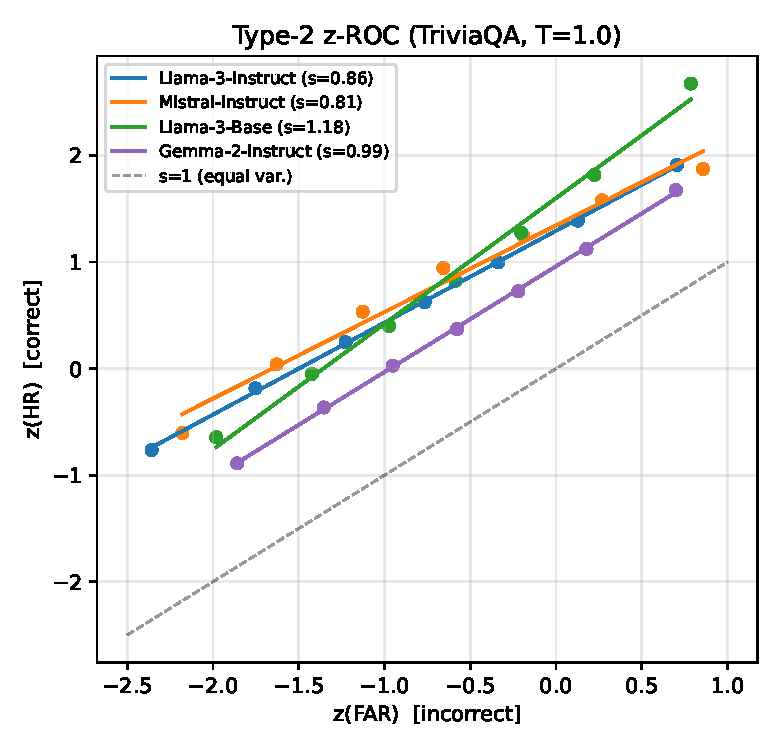
\includegraphics[width=0.5\textwidth]{fig_zroc.pdf}
\caption{Type-2 z-ROC (TriviaQA, $T{=}1.0$). Points are empirical (hit, false-alarm) pairs in probit coordinates; lines are SDT fits. Slopes below the equal-variance diagonal (Mistral, Llama-3-Instruct) indicate greater variance in correct-answer evidence.}
\label{fig:zroc}
\end{figure}

\subsection{Metacognitive information is decoupled from accuracy (H1, H4)}

\begin{table}[t]
\centering
\caption{Aggregate metacognition at $T{=}1.0$. meta-I$_{2r}$ is bias-corrected (permutation null subtracted); 95\% bootstrap CIs from 2{,}000 trial-level resamples. All meta-I$_{2r}$ exceed the permutation null ($p<0.001$). NQ column replicates the ordering.}
\label{tab:agg}
\small
\begin{tabular}{lccccc}
\toprule
\textbf{Model} & \textbf{Acc} & \textbf{meta-I$_{2r}$} & \textbf{95\% CI} & \textbf{AUROC$_2$} & \textbf{meta-I$_{2r}$ (NQ)} \\
\midrule
Mistral-Instruct & 0.427 & 0.328 & [0.307, 0.353] & 0.855 & 0.243 \\
Llama-3-Base & 0.428 & 0.292 & [0.273, 0.312] & 0.839 & 0.140 \\
Llama-3-Instruct & 0.543 & 0.276 & [0.256, 0.298] & 0.831 & 0.192 \\
Gemma-2-Instruct & 0.600 & 0.143 & [0.128, 0.161] & 0.747 & 0.108 \\
\bottomrule
\end{tabular}
\end{table}

Metacognitive information varies more than two-fold across models (meta-$I_{2r}$ 0.143--0.328 on TriviaQA; Table~\ref{tab:agg}) and is decoupled from accuracy. Mistral has the lowest accuracy (0.427) yet the highest metacognitive information (0.328, CI [0.307, 0.353]); Gemma-2, the most accurate (0.600), has the lowest (0.143, CI [0.128, 0.161]). The ordering is identical on Natural Questions, confirming a property of the confidence signal rather than of one dataset (Figure~\ref{fig:metai2r}). All four estimates exceed their permutation null ($p<0.001$).

\begin{figure}[t]
\centering
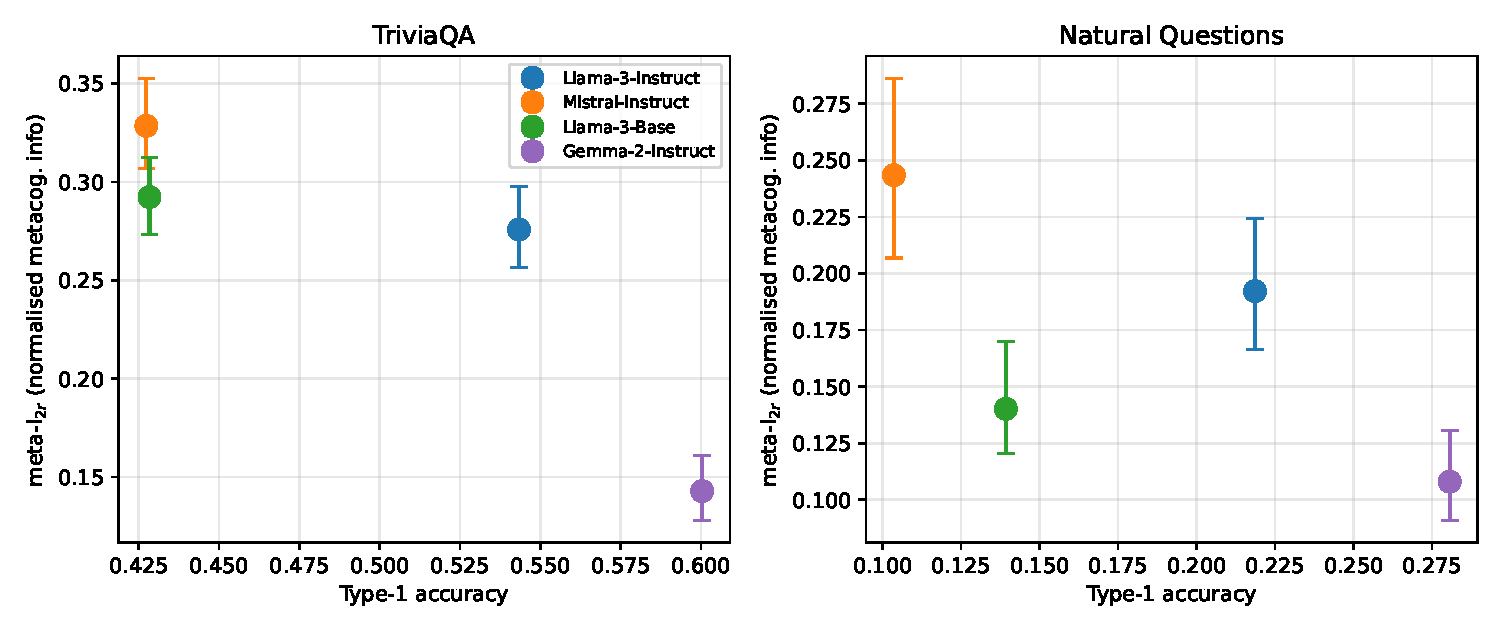
\includegraphics[width=\textwidth]{fig1_metai2r.pdf}
\caption{Metacognitive information vs.\ accuracy, both datasets. Error bars are 95\% bootstrap CIs. The least accurate model (Mistral) has the most informative confidence; the most accurate (Gemma-2) the least. Accuracy and metacognitive information are distinct axes of model quality.}
\label{fig:metai2r}
\end{figure}

A model can be highly accurate yet carry little usable confidence information (Gemma-2), or relatively inaccurate yet have confidence that sharply separates its own correct and incorrect answers (Mistral). This decoupling is invisible to accuracy, to ECE, and---because it does not normalise for accuracy---to raw AUROC$_2$ comparisons across models.

\subsection{Domain-specific metacognitive information (H2)}

\begin{table}[t]
\centering
\caption{Domain-specific meta-$I_{2r}$ at $T{=}1.0$ on TriviaQA. Boldface: weakest domain per model. Arts \& Literature is strongest for every model.}
\label{tab:domain}
\small
\begin{tabular}{lcccc}
\toprule
\textbf{Domain} & \textbf{Llama-Inst} & \textbf{Mistral} & \textbf{Base} & \textbf{Gemma} \\
\midrule
History \& Politics & 0.261 & 0.308 & 0.278 & 0.127 \\
Arts \& Literature & 0.326 & 0.337 & 0.330 & 0.194 \\
Geography & 0.248 & 0.315 & 0.260 & \textbf{0.065} \\
Science \& Technology & \textbf{0.162} & \textbf{0.286} & \textbf{0.240} & 0.084 \\
\bottomrule
\end{tabular}
\end{table}

\begin{figure}[t]
\centering
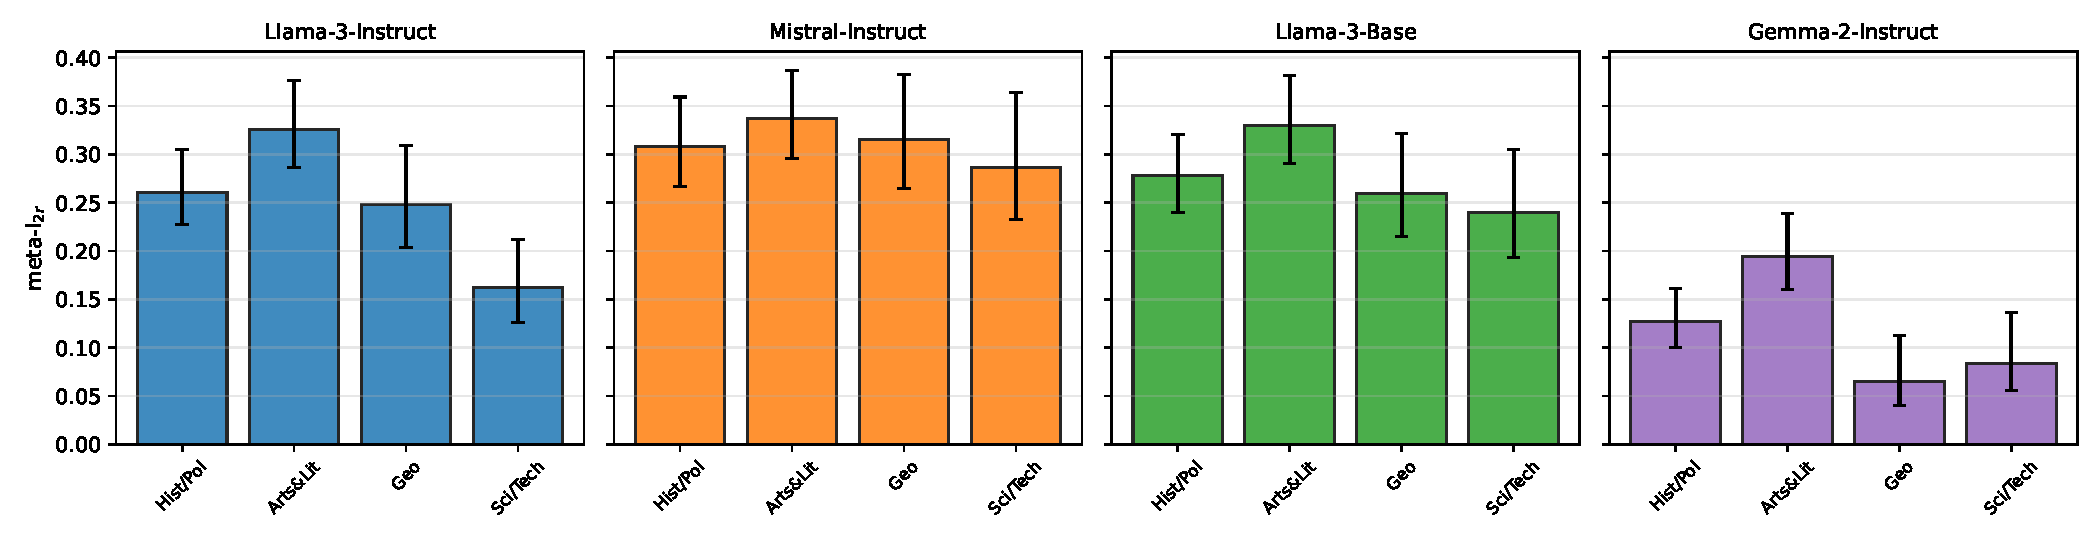
\includegraphics[width=\textwidth]{fig2_domain.pdf}
\caption{Domain-specific meta-$I_{2r}$ at $T{=}1.0$ on TriviaQA (95\% bootstrap CIs). Arts \& Literature is strongest for every model; the weakest domain is Science \& Technology or Geography.}
\label{fig:domain}
\end{figure}

Metacognitive information varies systematically across domains within each model (Table~\ref{tab:domain}, Figure~\ref{fig:domain}). Arts \& Literature is the strongest domain for all four models; the weakest is Science \& Technology (Llama-3-Instruct, Mistral, Llama-3-Base) or Geography (Gemma-2). The Llama-3-Instruct range across domains (0.162--0.326) is roughly double Mistral's (0.286--0.337): domain sensitivity of the confidence signal is itself model-dependent. A model whose confidence is informative in one domain and uninformative in another poses a deployment risk that aggregate metrics conceal.

\subsection{Temperature dissociates accuracy from metacognitive information (H3)}

\begin{figure}[t]
\centering

\includegraphics[width=\textwidth]{fig3_temperature.pdf}
\caption{meta-$I_{2r}$ (dashed) and accuracy (grey) vs.\ temperature on TriviaQA. Accuracy falls monotonically with temperature for all models; metacognitive information is near-flat for three of four, dissociating the two.}
\label{fig:temperature}
\end{figure}

Temperature dissociates Type-1 accuracy from metacognitive information (Figure~\ref{fig:temperature}). For all four models accuracy decreases monotonically with temperature (Spearman $\rho(\text{acc},T)=-1.00$). Metacognitive information is near-flat for three of four (meta-$I_{2r}$ range $\leq 0.025$ across $T\in\{0.3,0.5,0.7,1.0\}$ for Llama-3-Instruct, Mistral, and Gemma-2), moving in a different direction from accuracy. Llama-3-Base is the exception (range 0.101), the only model whose confidence informativeness changes materially with temperature. Temperature reshapes what a model gets right without, for most models, changing how well its confidence tracks correctness.

\subsection{Selective prediction (deployment consequence)}

The decoupling has a direct deployment consequence for selective prediction, where a system abstains on low-confidence responses. What metacognitive information predicts is the \emph{gain} from confidence-based selection, not the absolute accuracy attained---the latter is dominated by base accuracy. At 50\% coverage (accepting the top half of responses ranked by NLP), Mistral improves from 42.7\% to 70.7\% ($+28.0$ points) and Llama-3-Base from 42.8\% to 68.1\% ($+25.3$), while Gemma-2, with the least informative confidence, improves least relative to its accuracy (60.0\% to 77.4\%, $+17.4$). Across the four models, meta-$I_{2r}$ tracks the selective-prediction gain (Spearman $\rho=+0.80$) but not the accuracy level ($\rho=-0.60$), which follows base accuracy instead. A model with high accuracy but low metacognitive information (Gemma-2) reaches a high accuracy level under selection yet extracts little additional value from its own confidence; a model with lower accuracy but informative confidence (Mistral) benefits most from abstention. Neither pattern is visible from accuracy or ECE alone (full accuracy--coverage curves in Appendix~\ref{app:selective}).

% ════════════════════════════════════════════════════════════════
\section{Discussion}

\subsection{What an SDT analysis adds to LLM evaluation}

Confidence evaluation operates at three tiers. \emph{Tier~1} (ECE, Brier score) measures alignment, conflates sensitivity with bias, and is unstable under discretisation. \emph{Tier~2} (AUROC$_2$, rank correlations) measures ranking quality but does not normalise for accuracy, so it is not comparable across models of different accuracy. \emph{Tier~3} (meta-$I_{2r}$, and the z-ROC structure of the confidence signal) isolates how informative the confidence signal is about correctness, normalised for the base rate. Our results make the practical consequence concrete: Mistral has the lowest accuracy but the most informative confidence, and the confidence signals of different models have qualitatively different variance structure ($s$ from 0.81 to 1.18). Both facts are invisible to ECE.

\subsection{Temperature, criterion, and metacognitive capacity}

The dissociation between temperature and metacognitive information has implications for temperature tuning. For three of four models, temperature moves Type-1 accuracy without changing how well confidence tracks correctness. If a model's confidence is uninformative, lowering temperature to raise accuracy will not make its confidence more useful for selective prediction. For Llama-3-Base, where the dissociation does not hold, temperature does change the information content of confidence itself.

\subsection{Connections to human metacognition}

The phenomena parallel human metacognition, where metacognitive efficiency is domain-specific~\citep{rouault2018domain}, dissociable from Type-1 performance~\citep{fleming2010relating}, and neurally distinct from perceptual decisions~\citep{fleming2012prefrontal}. Our findings parallel these results functionally, not mechanistically: we do not claim LLMs possess metacognition phenomenologically. The measure differs from the human meta-$d'$ literature because open-ended QA lacks a Type-1 decision (\S\ref{sec:whynotmetad}); the value lies in the decomposition, consistent with the use of SDT in medical diagnosis~\citep{swets1996signal} and automated system evaluation~\citep{bartlett2017evaluating}.

\subsection{Limitations}
\label{sec:limitations}

Four open-weight 7--9B models; generalisability to frontier scale is unknown. API models that do not expose token-level log-probabilities cannot be evaluated with internal NLP; the verbal-confidence approach of \citet{dai2026rescaling} is a complementary path. All models ran as Q5\_K\_M quantisations; however, all measures depend on the \emph{ordinal} relationship between NLP and accuracy, which quantisation preserves, and the monotonicity check confirms this in all conditions. meta-$I_{2r}$ belongs to a family of information-theoretic metacognition measures~\citep{dayan2023metacognitive, fitousi2025information} with several normalisation choices; we use normalisation by accuracy entropy and report permutation nulls throughout to guard against the small-sample bias of plug-in mutual information. NLP is a fluency measure, not a pure metacognitive signal; a high meta-$I_{2r}$ does not imply the model ``knows that it knows'' in any deep sense.

\subsection{Recommendations for practice}
\begin{enumerate}[leftmargin=*, nosep]
    \item Report meta-$I_{2r}$ (with a permutation null) alongside ECE; they are complementary.
    \item Report the z-ROC slope of the confidence signal: unequal variance is a real, model-specific property.
    \item Disaggregate by domain; aggregate metrics hide domain-specific metacognitive deficits.
    \item For confidence-dependent systems, prefer higher metacognitive information over lower ECE.
    \item Evaluate temperature effects on metacognitive information, not just calibration.
\end{enumerate}

% ════════════════════════════════════════════════════════════════
\section{Conclusion}

We have applied Signal Detection Theory to LLM confidence, characterising the Type-2 ROC of the confidence signal and its unequal-variance structure, and---because the meta-$d'$ efficiency ratio is undefined for open-ended QA---quantifying metacognitive efficiency with a model-free information measure, meta-$I_{2r}$. Across four models and 224{,}000 trials, metacognitive information varies more than two-fold and is decoupled from accuracy: the least accurate model has the most informative confidence. The confidence signal has model-specific variance structure, efficiency is domain-specific, and temperature dissociates accuracy from metacognitive information. Current practice treats confidence as monolithic; an SDT decomposition shows this is insufficient. All analyses are pre-registered, with code and data publicly available.\footnote{Pre-registration: \url{https://osf.io/5q7mt}. Code and data: \url{https://github.com/synthiumjp/sdt_calibration}.}

\paragraph{Use of Generative AI.} Claude (Anthropic) was used as a research assistant for analysis pipeline design and code generation. All scientific decisions, hypothesis formulation, and interpretive judgments were made by the author.

\bibliographystyle{plainnat}
\bibliography{references}

% ════════════════════════════════════════════════════════════════
\appendix

\section{NLP Monotonicity Check}
\label{app:monotonicity}
Accuracy increases strictly across NLP quartiles in all eight model$\times$dataset conditions at $T{=}1.0$ (e.g., Gemma-2 on TriviaQA: $Q_1{=}0.314$, $Q_2{=}0.539$, $Q_3{=}0.690$, $Q_4{=}0.859$), validating NLP as a graded evidence variable.

\section{Selective Prediction: Accuracy--Coverage}
\label{app:selective}
Accuracy as a function of coverage (fraction of queries answered), abstaining on lowest-confidence responses. Models with higher meta-$I_{2r}$ obtain a larger accuracy \emph{gain} from confidence-based abstention (Spearman $\rho=+0.80$ between meta-$I_{2r}$ and the accuracy gain at 50\% coverage), while the absolute accuracy level under selection is governed by base accuracy. This confirms that metacognitive information predicts the value extracted from a model's own confidence signal, not the accuracy ceiling.

\end{document}
